\section{Erdos-Reyni Model}
\begin{definition}[Erdos-Reyni random graph]~

	Given $n \in \mathbb{Z}^+$ and a probability $p \in [0,1]$, the (E-R)
	random graph is denoted as $\mathcal{G}(n,p)$.
\end{definition}
\begin{itemize}
	\item The (RG) $\mathcal{G}(n,p)$ is undirected on all $n$ vertices
	\item Each of the $\binom{n}{2}$ edges is formed
	      independently from each other with probability $p$
	\item E-R stated a number of result that are based on "thresholds"
	      of $p$ which are needed to show the structural properties of
	      the graph:
	      \begin{enumerate}
		      \item $p$ is a function of $n$, $p \coloneq p(n)$
		      \item $\frac{1}{n^2}$ is the threshold for the first edges
		            to appear in a (RG)
		      \item $\frac{1}{n^{3/2}}$ is the threshold for the first
		            trees to emerge
		      \item $\frac{1}{n}$ is the threshold for the first cycles
		            to appear in the graph
	      \end{enumerate}
	\item If $p_{n} = 1/n$ then the "Giant component" emerges.
	      Let $p_{n} = (1-\varepsilon)/n$ for $0 < \varepsilon \ll 1)$,
	      then each "puddle" represents a region in the graph
	      where all nodes are connected.
	      \begin{center}
		      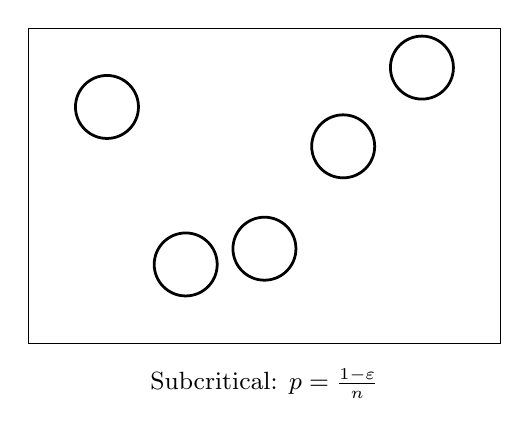
\begin{tikzpicture}
			      % bounding box
			      \draw (0,0) rectangle (6,4);
			      % small puddles
			      \foreach \x/\y in {1/3,2/1,4/2.5,5/3.5,3/1.2}{
					      \draw[line width=1pt] (\x,\y) circle (0.4);
				      }
			      \node[below=2mm] at (3,0) {\small Subcritical: $p=\frac{1-\varepsilon}{n}$};
		      \end{tikzpicture}
	      \end{center}
	      Note that $p_{n}$ is to the left of $\varepsilon$ and that
	      the size of the largest puddles are "small",
	      $\to O(\log n)$ w.h.p.
	\item For $p_{n} = (1+\varepsilon) / n$, we go to the
	      right of $\varepsilon \to 1 + \varepsilon$.
	      \begin{center}
		      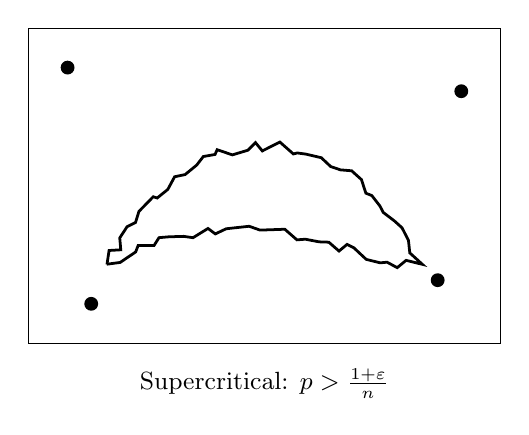
\begin{tikzpicture}
			      % bounding box
			      \draw (0,0) rectangle (6,4);

			      % giant component (irregular blob)
			      \draw[
				      line width=1pt,
				      decorate,
				      decoration={random steps,segment length=4pt,amplitude=2pt}
			      ] (1,1) .. controls (2,3) and (4,3) .. (5,1)
			      .. controls (4,1) and (3,2) .. (1,1)
			      -- cycle;

			      % isolated nodes
			      \foreach \x/\y in {0.5/3.5,5.5/3.2,5.2/0.8,0.8/0.5}{
					      \fill (\x,\y) circle (2.5pt);
				      }

			      % caption
			      \node[below=2mm] at (3,0)
			      {\small Supercritical: \(p > \frac{1+\varepsilon}{n}\)};
		      \end{tikzpicture}
	      \end{center}
	      Here we have one large "island" where it's size is
	      relatively, $O(n)$ w.h.p.
\end{itemize}
